\section{Results and Analysis}
\label{sec:results}

% ---------------------------------------------------------------------------------- A
\subsection{Dataset Description}
\label{sec:dataset}

All experiments use PTB-XL v1.0.3 \cite{wagner2020ptbxl}, an open-access (CC BY 4.0) collection
distributed through PhysioNet \cite{goldberger2000}. It contains 21,799 clinical 12-lead ECGs of
10~s from 18,869 patients, recorded with Schiller devices and annotated with SCP-ECG statements by
up to two cardiologists; the 100-Hz version of the waveforms is used here. As described in
Section~\ref{sec:prep}, 411 records without a diagnostic superclass were removed, leaving 21,388
records from 18,617 patients. The mean age of the retained patients is 59.4 $\pm$ 16.8 years
(ages above 89 are stored as a placeholder in PTB-XL and were excluded from this mean), and 48.1\%
of the records belong to female patients. The labels are the five diagnostic superclasses: normal
ECG (NORM), myocardial infarction (MI), ST/T change (STTC), conduction disturbance (CD) and
hypertrophy (HYP). Because a recording may carry several superclasses, the mean number of labels per
record is 1.30 and 24.1\% of the records are multi-label.

The official stratified folds of PTB-XL were used without modification, which guarantees that all
recordings of a patient lie in a single fold. Folds 1--8 (17,084 records, 80\%) form the training
data and are divided among the four clients, fold 9 (2,146 records, 10\%) is the validation set
used for early stopping, calibration, thresholds and the gate, and fold 10 (2,158 records from
1,877 patients, 10\%) is the test set. The split is therefore 80/10/10 rather than 80/20: the
separate validation fold prevents any model or gate choice from being tuned on the test data.
Table~\ref{tab:dataset} lists the records, patients and class counts of every partition, and
Fig.~\ref{fig:classdist} shows the class distribution. NORM is the most frequent superclass
(44.5\% of records) and HYP the rarest (12.4\%), and the class proportions of the four clients
differ by less than one percentage point.

\begin{table*}[!t]
\centering
\caption{Dataset details: records, patients and positive labels per partition (prevalence in \% in parentheses)}
\label{tab:dataset}
\footnotesize
\begin{tabular}{@{}lcccccccc@{}}
\toprule
Partition & Folds & Records & Patients & NORM & MI & STTC & CD & HYP \\
\midrule
Client A & 1, 2 & 4{,}277 & 3{,}676 & 1{,}907 & 1{,}087 & 1{,}050 & 966 & 527 \\
Client B & 3, 4 & 4{,}280 & 3{,}722 & 1{,}918 & 1{,}079 & 1{,}042 & 981 & 525 \\
Client C & 5, 6 & 4{,}264 & 3{,}725 & 1{,}869 & 1{,}125 & 1{,}060 & 990 & 535 \\
Client D & 7, 8 & 4{,}263 & 3{,}700 & 1{,}902 & 1{,}088 & 1{,}034 & 970 & 532 \\
\midrule
Train & 1--8 & 17{,}084 & 14{,}823 & 7{,}596 (44.5) & 4{,}379 (25.6) & 4{,}186 (24.5) & 3{,}907 (22.9) & 2{,}119 (12.4) \\
Validation & 9 & 2{,}146 & 1{,}917 & 955 (44.5) & 540 (25.2) & 528 (24.6) & 495 (23.1) & 268 (12.5) \\
Test & 10 & 2{,}158 & 1{,}877 & 963 (44.6) & 550 (25.5) & 521 (24.1) & 496 (23.0) & 262 (12.1) \\
\midrule
Total & 1--10 & 21{,}388 & 18{,}617 & 9{,}514 (44.5) & 5{,}469 (25.6) & 5{,}235 (24.5) & 4{,}898 (22.9) & 2{,}649 (12.4) \\
\bottomrule
\end{tabular}

\end{table*}

\begin{figure}[!t]
\centering
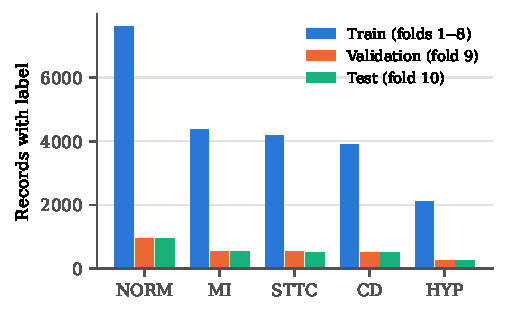
\includegraphics[width=\columnwidth]{class_distribution}
\caption{Number of records carrying each diagnostic superclass in the training, validation and test
folds (multi-label, so a record can be counted in several classes).}
\label{fig:classdist}
\end{figure}

% ---------------------------------------------------------------------------------- B
\subsection{Experimental Setup}
\label{sec:setup}

All networks were implemented in PyTorch \cite{paszke2019pytorch} and trained on an Apple M1
MacBook Air with 8~GB of unified memory using the Metal (MPS) backend, under macOS, Python 3.11.17 and PyTorch 2.14.1. Mixed precision was not
used. A mean training epoch took 26.8~s for Client~A, 38.5~s for Client~B, 65.4~s for Client~C and
28.2~s for Client~D. Every experiment was repeated with the random seeds 42, 43 and 44, and results
are reported as mean $\pm$ standard deviation over the three seeds. Table~\ref{tab:hyper} lists all
hyperparameters; they are identical for every client so that only the architecture and the data
differ.

\begin{table}[!t]
\centering
\caption{Hyperparameters}
\label{tab:hyper}
\footnotesize
\begin{tabular}{@{}p{3.3cm}p{4.7cm}@{}}
\toprule
Parameter & Value \\
\midrule
Input & $12\times1000$ (10 s at 100 Hz) \\
Number of clients & 4 (A, B, C, D), 2 PTB-XL folds each \\
Communication rounds & 1 (one-shot; probabilities only) \\
Local epochs & up to 50; early stopping, patience 8 \\
Early-stopping criterion & macro AUROC on fold 9 \\
Batch size & 128 \\
Optimizer & AdamW \cite{loshchilov2019adamw}, weight decay $10^{-2}$ \\
Learning rate & $10^{-3}$, OneCycle schedule \cite{smith2019superconvergence} \\
Loss & BCE with logits, positive weight $N^-_c/N^+_c$ \\
Gradient clipping & global norm 1.0 \\
Head & Linear 256, ReLU, dropout 0.3, Linear 5 \\
Activation & ReLU (BiLSTM: sigmoid/tanh gates) \\
Calibration & 1 temperature per client, LBFGS on fold 9 \\
Aggregation & equal / static / dynamic gate; selection by 5-fold patient-grouped CV, margin 0.002 \\
Static gate & 4 weights, Adam lr 0.05, 500 steps \\
Dynamic gate & MLP 24--32--4, dropout 0.2, AdamW lr $10^{-3}$, $\le$300 epochs, patience 30 \\
Thresholds & per class, max.\ F1 on fold 9 \\
Bootstrap & 1,000 resamples (95\% CI, paired) \\
Seeds & 42, 43, 44 \\
\bottomrule
\end{tabular}
\end{table}

Because the task is multi-label, every metric is first computed per class from that class's
confusion counts $TP_c$, $FP_c$, $FN_c$ and $TN_c$ on the $N$ test records, and then macro-averaged
over the five classes:
\begin{align}
\mathrm{Precision}_c &= \frac{TP_c}{TP_c+FP_c},\qquad \mathrm{Recall}_c = \frac{TP_c}{TP_c+FN_c},\\
\mathrm{Specificity}_c &= \frac{TN_c}{TN_c+FP_c},\\
\mathrm{F1}_c &= \frac{2\,\mathrm{Precision}_c\,\mathrm{Recall}_c}{\mathrm{Precision}_c+\mathrm{Recall}_c},\\
\mathrm{Acc}_{\text{label}} &= \frac{1}{5}\sum_{c=1}^{5}\frac{TP_c+TN_c}{N},\\
\mathrm{Acc}_{\text{exact}} &= \frac{1}{N}\sum_{n=1}^{N}\big[\mathbf y^{\mathrm{pred}}_n=\mathbf y_n\big].
\end{align}
Label-wise accuracy (reported as ``Acc.'') counts every one of the five decisions per record, whereas
exact-match accuracy requires all five decisions of a record to be correct. The area under the ROC
curve is $\mathrm{AUROC}_c=\int_0^1\mathrm{TPR}_c\,d\,\mathrm{FPR}_c$, the probability that a random
positive is ranked above a random negative, and is threshold-free; AUPRC is the area under the
precision--recall curve. Macro AUROC is the primary metric, because it is insensitive to the
decision thresholds and to class prevalence, and its 95\% confidence interval is obtained with 1,000
bootstrap resamples of the test records \cite{efron1993bootstrap}. Differences between two models are
assessed with a paired bootstrap on the same resamples. Regression metrics (MAE, RMSE, $R^2$) do not
apply because the task has no continuous target (Section~\ref{sec:clf}).

% ---------------------------------------------------------------------------------- C
\subsection{Comparison of Performance Metrics With Traditional Machine Learning Models and Unimodal Models}
\label{sec:comparison}

Table~\ref{tab:main} compares the proposed model with the individual deep clients, with the two
learned aggregation variants and with a centrally trained reference. All rows were evaluated once
on the same test fold with thresholds chosen on fold 9. The traditional classifiers use 172
hand-crafted features computed from the filtered, un-normalised signal: per-lead amplitude statistics
(standard deviation, minimum, maximum, range, skewness, kurtosis, mean absolute slope), relative
spectral power in the 0.5--5, 5--15 and 15--40~Hz bands, heart rate and RR-interval variability from
R peaks detected in lead II, and per-lead median R, S, ST and T amplitudes around those peaks. They
were trained on the pooled folds 1--8, Platt-scaled on fold 9 and thresholded on fold 9 like the deep
models; Random Forest and XGBoost were run with the three seeds, while logistic regression, the RBF SVM
and KNN are deterministic.

\begin{table*}[!t]
\centering
\caption{Comparison with traditional machine-learning models, the individual deep clients and the
aggregation variants on the PTB-XL test fold (mean $\pm$ SD over 3 seeds; Acc.\ = label-wise
accuracy; Prec., Rec., F1, AUROC and AUPRC are macro averages over the five superclasses)}
\label{tab:main}
\footnotesize
\begin{tabular}{@{}llcccccc@{}}
\toprule
Model & Params & Acc. (\%) & Prec. (\%) & Rec. (\%) & F1 (\%) & AUROC & AUPRC \\
\midrule
\multicolumn{8}{@{}l}{\emph{Traditional machine learning (172 hand-crafted features, pooled folds 1--8)}}\\
Logistic Regression & -- & 84.4 $\pm$ 0.0 & 65.3 $\pm$ 0.0 & 71.7 $\pm$ 0.0 & 68.2 $\pm$ 0.0 & 0.880 $\pm$ 0.000 & 0.724 $\pm$ 0.000 \\
SVM (RBF) & -- & 85.8 $\pm$ 0.0 & 67.3 $\pm$ 0.0 & 74.5 $\pm$ 0.0 & 70.6 $\pm$ 0.0 & 0.898 $\pm$ 0.000 & 0.772 $\pm$ 0.000 \\
Random Forest & -- & 86.2 $\pm$ 0.2 & 69.1 $\pm$ 0.8 & 74.0 $\pm$ 1.2 & 71.2 $\pm$ 0.2 & 0.902 $\pm$ 0.001 & 0.778 $\pm$ 0.001 \\
KNN & -- & 82.2 $\pm$ 0.0 & 60.8 $\pm$ 0.0 & 68.9 $\pm$ 0.0 & 64.4 $\pm$ 0.0 & 0.859 $\pm$ 0.000 & 0.700 $\pm$ 0.000 \\
XGBoost & -- & 86.8 $\pm$ 0.0 & 69.7 $\pm$ 0.2 & 76.3 $\pm$ 0.5 & 72.6 $\pm$ 0.2 & 0.909 $\pm$ 0.002 & 0.789 $\pm$ 0.003 \\
\midrule
\multicolumn{8}{@{}l}{\emph{Single deep clients (25\% of training data each)}}\\
Client A: 1D CNN & 0.44M & 84.8 $\pm$ 0.2 & 64.6 $\pm$ 0.6 & 72.6 $\pm$ 0.8 & 68.0 $\pm$ 0.3 & 0.888 $\pm$ 0.002 & 0.738 $\pm$ 0.005 \\
Client B: 1D ResNet & 6.73M & 84.0 $\pm$ 0.8 & 63.0 $\pm$ 1.3 & 73.4 $\pm$ 1.8 & 67.2 $\pm$ 0.4 & 0.882 $\pm$ 0.002 & 0.721 $\pm$ 0.005 \\
Client C: BiLSTM & 0.67M & 85.5 $\pm$ 0.3 & 66.2 $\pm$ 1.2 & 73.3 $\pm$ 0.5 & 69.2 $\pm$ 0.3 & 0.894 $\pm$ 0.000 & 0.745 $\pm$ 0.003 \\
Client D: CNN-LSTM & 0.47M & 85.7 $\pm$ 0.8 & 67.0 $\pm$ 2.8 & 72.2 $\pm$ 3.1 & 69.0 $\pm$ 0.1 & 0.896 $\pm$ 0.001 & 0.749 $\pm$ 0.006 \\
\midrule
\multicolumn{8}{@{}l}{\emph{Aggregation of the four clients}}\\
Static learned weights & 4 & 86.6 $\pm$ 0.3 & 68.5 $\pm$ 0.9 & 72.8 $\pm$ 0.8 & 70.3 $\pm$ 0.3 & 0.903 $\pm$ 0.001 & 0.764 $\pm$ 0.004 \\
Dynamic gate & $\approx$1k & 86.4 $\pm$ 0.3 & 68.1 $\pm$ 1.2 & 72.9 $\pm$ 1.3 & 70.2 $\pm$ 0.1 & 0.901 $\pm$ 0.001 & 0.759 $\pm$ 0.002 \\
\textbf{Proposed (equal-weight gate)} & 8.31M & 86.9 $\pm$ 0.2 & 69.8 $\pm$ 0.9 & 72.5 $\pm$ 2.1 & 70.7 $\pm$ 0.6 & 0.905 $\pm$ 0.000 & 0.767 $\pm$ 0.002 \\
\midrule
\multicolumn{8}{@{}l}{\emph{Centralised reference (data pooled, not federated)}}\\
CNN-LSTM on folds 1--8 & 0.47M & 86.4 $\pm$ 0.7 & 68.5 $\pm$ 1.2 & 74.0 $\pm$ 0.6 & 70.7 $\pm$ 0.8 & 0.909 $\pm$ 0.001 & 0.774 $\pm$ 0.002 \\
\bottomrule
\end{tabular}

\end{table*}

The four deep clients, each trained on only a quarter of the training data, reach test macro AUROCs
between 0.882 (Client B, 1D ResNet) and 0.896 (Client D, CNN-LSTM). The recurrent clients rank best:
the BiLSTM (0.894) and the CNN-LSTM (0.896) outperform both convolutional clients, and the ResNet,
despite having the most parameters (6.73M), is the weakest, which is consistent with its early
stopping after 13.7 epochs on average (Table~\ref{tab:clienttrain}) and indicates over-fitting on
4,280 records. The proposed equal-weight gate raises the macro AUROC to 0.905 $\pm$ 0.000, the
label-wise accuracy to 86.9\% (from at most 85.7\%), the macro F1 to 70.7\% (from at most 69.2\%)
and the macro precision to 69.8\% (from at most 67.0\%), while keeping the recall (72.5\%) at the
level of the clients. Its AUPRC of 0.767 is also the highest among the federated models. A CNN-LSTM
trained centrally on all eight training folds, which is not possible when the data cannot be pooled,
attains 0.909 $\pm$ 0.001 macro AUROC and the same macro F1 of 70.7\%; the federated gate therefore
recovers about 70\% of the AUROC lost by splitting the data (0.896 $\rightarrow$ 0.905 of the
0.896 $\rightarrow$ 0.909 gap) and is tied with the pooled model in F1. As an external reference for
feature-based learning on the same test fold, the wavelet-feature neural network of
\cite{strodthoff2021} reported a superdiagnostic macro AUROC of 0.874.

The traditional classifiers turn out to be strong baselines. Trained on all pooled data, XGBoost
reaches a macro AUROC of 0.909 $\pm$ 0.002 and a macro F1 of 72.6\%, and Random Forest 0.902 and
71.2\%, so the best of them matches the pooled CNN-LSTM in AUROC and exceeds both it and the
federated gate in F1; KNN (0.859) and logistic regression (0.880) are clearly weaker. The amplitude
features are the likely reason: they keep the absolute voltages that the per-recording z-scoring of
the deep models removes, and these voltages define hypertrophy. The comparison is, however, not a
federated one, because these models see four times as much data as each client. Table~\ref{tab:tradlocal}
therefore trains the same classifiers on a single client's two folds. Under this restriction XGBoost
reaches 0.898 on average and Random Forest 0.893--0.895, i.e.\ the level of the best deep clients
(0.894--0.896), and every locally trained model, traditional or deep, remains below the federated
gate (0.905).

\begin{table}[!t]
\centering
\caption{Traditional classifiers trained locally (one client's folds; mean $\pm$ SD over clients A--D,
seed 42) or on pooled data (mean $\pm$ SD over 3 seeds), compared with the best deep clients (test fold)}
\label{tab:tradlocal}
\footnotesize
\setlength{\tabcolsep}{3pt}
\resizebox{\columnwidth}{!}{\begin{tabular}{@{}lcccc@{}}
\toprule
 & \multicolumn{2}{c}{Local (one client, mean of A--D)} & \multicolumn{2}{c}{Pooled (folds 1--8)} \\
\cmidrule(lr){2-3}\cmidrule(l){4-5}
Model & AUROC & F1 (\%) & AUROC & F1 (\%) \\
\midrule
Logistic Regression & 0.870 $\pm$ 0.001 & 67.0 $\pm$ 0.1 & 0.880 $\pm$ 0.000 & 68.2 $\pm$ 0.0 \\
SVM (RBF) & 0.886 $\pm$ 0.002 & 68.8 $\pm$ 0.3 & 0.898 $\pm$ 0.000 & 70.6 $\pm$ 0.0 \\
Random Forest & 0.894 $\pm$ 0.001 & 69.8 $\pm$ 0.2 & 0.902 $\pm$ 0.001 & 71.2 $\pm$ 0.2 \\
KNN & 0.847 $\pm$ 0.004 & 63.3 $\pm$ 0.6 & 0.859 $\pm$ 0.000 & 64.4 $\pm$ 0.0 \\
XGBoost & 0.898 $\pm$ 0.002 & 70.4 $\pm$ 0.4 & 0.909 $\pm$ 0.002 & 72.6 $\pm$ 0.2 \\
\midrule
Deep client C (BiLSTM) & 0.894 $\pm$ 0.000 & 69.2 $\pm$ 0.3 & -- & -- \\
Deep client D (CNN-LSTM) & 0.896 $\pm$ 0.001 & 69.0 $\pm$ 0.1 & -- & -- \\
\bottomrule
\end{tabular}
}
\end{table}

The study uses a single input modality, the 12-lead ECG, so a comparison of unimodal and multimodal
models in the strict sense is not possible. Table~\ref{tab:clientgate} instead contrasts each
single-architecture client with the federated combination of all four, per superclass. The gate
achieves the highest AUROC in every class, and its largest gain over the best client is observed for
the hardest class, HYP (0.828 versus at most 0.809). This indicates that the clients make partly
independent errors that the combination averages out, the same mechanism that motivates
multimodal fusion, but obtained here from architectural rather than modal diversity.

\begin{table}[!t]
\centering
\caption{Single clients versus the federated gate: test AUROC per superclass (mean of 3 seeds; best in bold)}
\label{tab:clientgate}
\footnotesize
\setlength{\tabcolsep}{3.5pt}
\begin{tabular}{@{}lccccc|c@{}}
\toprule
Model & NORM & MI & STTC & CD & HYP & Macro \\
\midrule
Client A (1D CNN) & 0.926 & 0.891 & 0.925 & 0.900 & 0.798 & 0.888 \\
Client B (1D ResNet) & 0.922 & 0.877 & 0.918 & 0.884 & 0.808 & 0.882 \\
Client C (BiLSTM) & 0.931 & 0.901 & 0.926 & 0.902 & 0.809 & 0.894 \\
Client D (CNN-LSTM) & 0.933 & 0.906 & 0.923 & 0.909 & 0.808 & 0.896 \\
\textbf{Proposed} & \textbf{0.938} & \textbf{0.912} & \textbf{0.933} & \textbf{0.914} & \textbf{0.828} & 0.905 \\
\bottomrule
\end{tabular}

\end{table}

The gain over the best single client is statistically significant. In a paired bootstrap on the test
fold, the macro AUROC of the gate exceeds that of the best client chosen on fold 9 by +0.012
[+0.009, +0.016] for seed 42 (Client C), +0.011 [+0.007, +0.014] for seed 43 (Client C) and +0.009
[+0.005, +0.013] for seed 44 (Client D), so every confidence interval lies above zero. The macro F1
improves by +0.018 [+0.009, +0.028], +0.010 [$-$0.001, +0.021] and +0.024 [+0.014, +0.034],
respectively, with the interval excluding zero in two of the three seeds. Fig.~\ref{fig:modelcomp}
summarises the macro AUROC of all models.

\begin{figure}[!t]
\centering
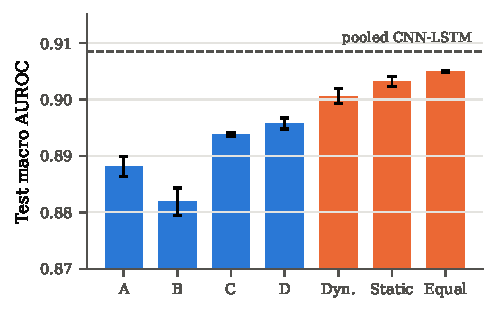
\includegraphics[width=\columnwidth]{model_comparison}
\caption{Test macro AUROC of the four clients and the three aggregation variants (mean $\pm$ SD over
3 seeds). The dashed line marks the centrally trained CNN-LSTM.}
\label{fig:modelcomp}
\end{figure}

% ---------------------------------------------------------------------------------- D
\subsection{Ablation Experiments}
\label{sec:ablation}

\subsubsection{Modality Ablation Experiment}
Since the ECG is the only modality, the input-source ablation was carried out over the
participating institutions: every one of the 15 non-empty subsets of $\{A,B,C,D\}$ was combined with
equal weights and evaluated on fold 9 (cross-validated) and on the test fold. The results, ordered by
the number of clients, are given in Table~\ref{tab:subsets}, and Table~\ref{tab:shapley} converts them
into a Shapley value per client.
\begin{table}[!t]
\centering
\caption{Client-subset ablation (equal-weight gate; mean over 3 seeds, test SD shown)}
\label{tab:subsets}
\footnotesize
\setlength{\tabcolsep}{4pt}
\begin{tabular}{@{}clccc@{}}
\toprule
\#Clients & Subset & Fold-9 CV AUROC & Test AUROC & $\Delta$ vs.\ ABCD \\
\midrule
4 & \textbf{ABCD} & 0.909 & 0.905 $\pm$ 0.000 & 0.000 \\
\midrule
3 & ACD & 0.908 & 0.905 $\pm$ 0.000 & 0.000 \\
3 & BCD & 0.908 & 0.904 $\pm$ 0.001 & -0.001 \\
3 & ABC & 0.906 & 0.901 $\pm$ 0.000 & -0.004 \\
3 & ABD & 0.905 & 0.902 $\pm$ 0.001 & -0.003 \\
\midrule
2 & CD & 0.907 & 0.903 $\pm$ 0.001 & -0.002 \\
2 & AC & 0.905 & 0.900 $\pm$ 0.000 & -0.005 \\
2 & AD & 0.904 & 0.901 $\pm$ 0.001 & -0.004 \\
2 & BC & 0.903 & 0.898 $\pm$ 0.001 & -0.007 \\
2 & BD & 0.903 & 0.900 $\pm$ 0.001 & -0.005 \\
2 & AB & 0.899 & 0.895 $\pm$ 0.001 & -0.010 \\
\midrule
1 & C & 0.900 & 0.894 $\pm$ 0.000 & -0.011 \\
1 & D & 0.898 & 0.896 $\pm$ 0.001 & -0.009 \\
1 & A & 0.893 & 0.888 $\pm$ 0.002 & -0.017 \\
1 & B & 0.886 & 0.882 $\pm$ 0.003 & -0.023 \\
\bottomrule
\end{tabular}

\end{table}

The full federation ABCD is the best configuration on both splits (fold 9: 0.909; test: 0.905).
Every two-client combination outperforms every single client on the test fold, so most of the gain
comes from combining heterogeneous models at all, and adding clients yields diminishing returns
(single: at most 0.896; pairs: at most 0.903; triples: at most 0.905). Removing the recurrent clients
hurts most: dropping D lowers the test AUROC by 0.004 and dropping C by 0.003, whereas dropping A or B
costs at most 0.001. The Shapley values in Table~\ref{tab:shapley} confirm this ranking (C and D
largest, B smallest), but they also show that the four contributions are of the same order
(0.097--0.105 on the test fold). This explains why equal weighting works well: the learned static
weights assign almost nothing to Client A (0.001 on average), although its marginal contribution to
the federation is comparable to that of the other clients.

\begin{table}[!t]
\centering
\caption{Shapley value $\phi_i$ of each client for the macro AUROC of the equal-weight federation
($v(\emptyset)=0.5$) and the mean learned static weight}
\label{tab:shapley}
\footnotesize
\setlength{\tabcolsep}{4pt}
\begin{tabular}{@{}lcccc@{}}
\toprule
Client & Architecture & $\phi$ (fold 9) & $\phi$ (test) & Static weight $w_i$ \\
\midrule
A & 1D CNN & 0.1009 & 0.0998 & 0.001 \\
B & 1D ResNet & 0.0980 & 0.0971 & 0.042 \\
C & BiLSTM & 0.1055 & 0.1033 & 0.549 \\
D & CNN-LSTM & 0.1043 & 0.1047 & 0.407 \\
\midrule
Sum & -- & 0.4087 & 0.4050 & 1.000 \\
\bottomrule
\end{tabular}

\end{table}

\subsubsection{Feature Fusion Module Ablation Experiments}
Table~\ref{tab:fusion} compares the three fusion strategies of Section~\ref{sec:fl}: equal weights,
learned static weights and the dynamic per-patient gate. All three are late (decision-level) fusion
strategies, because the clients do not share embeddings; early or feature-level fusion is excluded by
the privacy constraint. The validation columns are the patient-grouped cross-validated values used for
selection, and the test columns were obtained afterwards.

\begin{table*}[!t]
\centering
\caption{Ablation of the fusion strategy (fold-9 CV values used for selection; test values mean $\pm$ SD over 3 seeds)}
\label{tab:fusion}
\footnotesize
\begin{tabular}{@{}lccccc@{}}
\toprule
Fusion strategy & CV AUROC & CV BCE & Test AUROC & Test F1 (\%) & Exact match (\%) \\
\midrule
\textbf{Equal weights (selected)} & 0.909 & 0.372 & 0.905 $\pm$ 0.000 & 70.7 $\pm$ 0.6 & 58.1 $\pm$ 0.7 \\
Static learned weights & 0.907 & 0.346 & 0.903 $\pm$ 0.001 & 70.3 $\pm$ 0.3 & 57.0 $\pm$ 1.5 \\
Dynamic per-patient gate & 0.904 & 0.338 & 0.901 $\pm$ 0.001 & 70.2 $\pm$ 0.1 & 56.8 $\pm$ 0.7 \\
\bottomrule
\end{tabular}

\end{table*}

Equal weights achieve the highest cross-validated macro AUROC (0.909) and were selected in all three
seeds; learned static weights (0.907) and the dynamic gate (0.904) did not reach the required
margin. The learned combiners achieve a lower cross-validated binary cross-entropy (0.346 and 0.338
versus 0.372), i.e.\ they produce better-calibrated probabilities, but they do so by concentrating
the weight on Clients C and D (Fig.~\ref{fig:weights}), which sacrifices the diversity contributed by
A and B and lowers the ranking quality. The dynamic gate never outperformed the simpler combiners: its
per-patient weights differ little from the static ones (mean test weights 0.002, 0.092, 0.532 and
0.374 for A--D), because all clients receive the same ECG and there is little patient-specific
information about which client to trust. The same ordering holds on the test fold (0.905, 0.903 and
0.901), so the selection made on validation data was confirmed.

\begin{figure}[!t]
\centering
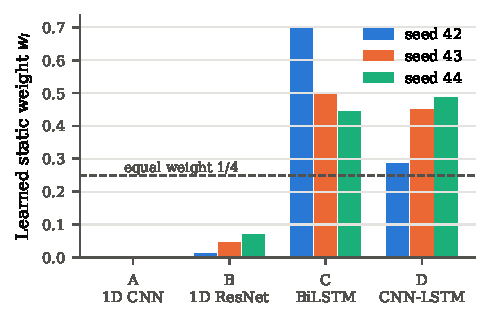
\includegraphics[width=\columnwidth]{weights}
\caption{Static aggregation weights learned on fold 9 for each seed. The dashed line marks the equal
weight 1/4 used by the selected gate.}
\label{fig:weights}
\end{figure}

\subsubsection{Ablation Study on Activation Function and Optimizer}
The choice of activation function and optimizer was examined on Client~D (CNN-LSTM, folds 7--8, seed
42), keeping every other element of the recipe fixed, including the OneCycle schedule with a maximum
learning rate of $10^{-3}$, early stopping on fold 9 and the class-weighted loss. To avoid any tuning
on the test data, the ablations were evaluated on fold 9 only. In the activation ablation the ReLU of
the convolutional blocks and of the classification head was replaced, while the gates of the LSTM were
left unchanged. Tables~\ref{tab:act} and~\ref{tab:opt} report the best fold-9 macro AUROC, the epoch at
which it was reached, the number of epochs before early stopping and the training loss at the selected
epoch.

\begin{table}[!t]
\centering
\caption{Activation-function ablation (Client D, CNN-LSTM, seed 42; fold-9 macro AUROC)}
\label{tab:act}
\footnotesize
\resizebox{\columnwidth}{!}{\begin{tabular}{@{}lccc@{}}
\toprule
Activation & Fold-9 AUROC & Best / run epochs & Train loss \\
\midrule
ReLU (used) & 0.898 & 23 / 31 & 0.444 \\
LeakyReLU & \textbf{0.898} & 24 / 32 & 0.423 \\
ELU & 0.895 & 14 / 22 & 0.547 \\
GELU & 0.896 & 14 / 22 & 0.534 \\
Tanh & 0.894 & 19 / 27 & 0.484 \\
\bottomrule
\end{tabular}
}
\end{table}

\begin{table}[!t]
\centering
\caption{Optimizer ablation (Client D, CNN-LSTM, seed 42; fold-9 macro AUROC; maximum learning rate
$10^{-3}$ for all optimizers)}
\label{tab:opt}
\footnotesize
\resizebox{\columnwidth}{!}{\begin{tabular}{@{}lccc@{}}
\toprule
Optimizer & Fold-9 AUROC & Best / run epochs & Train loss \\
\midrule
AdamW (used) & \textbf{0.898} & 23 / 31 & 0.444 \\
Adam \cite{kingma2015adam} & 0.898 & 20 / 28 & 0.480 \\
SGD (momentum 0.9) & 0.786 & 30 / 38 & 1.014 \\
RMSprop (momentum 0.9) & 0.855 & 3 / 11 & 0.724 \\
\bottomrule
\end{tabular}
}
\end{table}

ReLU and LeakyReLU perform identically (0.898), and they also train longest before early stopping (23
and 24 epochs to the best model), reaching the lowest training losses (0.444 and 0.423). The smooth
activations GELU (0.896) and ELU (0.895) converge faster, with their best epoch at 14, but to a
slightly lower AUROC, and the saturating tanh is the weakest (0.894). The differences are at most 0.004
AUROC, so the activation function is not a decisive design factor for this model, and the ReLU used for
all clients is among the best choices.

The optimizer matters much more. AdamW and Adam reach the same AUROC (0.898), which shows that the
decoupled weight decay neither helped nor hurt at this data size. SGD with momentum is clearly
inferior (0.786): with the same maximum learning rate of $10^{-3}$ it was still improving slowly when
it stopped after 38 epochs, with a training loss of 1.014, so it would need a much larger learning rate
or longer training. RMSprop reached its best AUROC of 0.855 already at epoch 3 and did not improve
afterwards, which indicates unstable optimisation with this learning rate and momentum. Adaptive
moment-based optimizers are therefore the appropriate choice for the clients, and the configuration
used in this work (ReLU with AdamW) is confirmed by both ablations.

% ---------------------------------------------------------------------------------- E
\subsection{Federated Learning Results Analysis}
\label{sec:flresults}

\subsubsection{Client-wise Training Accuracy and Loss}
Because the federation consists of a single round, the training dynamics of the system are those
of the four local trainings. Fig.~\ref{fig:clientcurves} shows, for seed 42, the validation macro
AUROC (the early-stopping criterion, used here in place of accuracy because the label-wise accuracy
depends on thresholds that are fitted only after training) and the weighted training loss of every
client over its local epochs, and Table~\ref{tab:clienttrain} summarises all three seeds.

\begin{figure*}[!t]
\centering
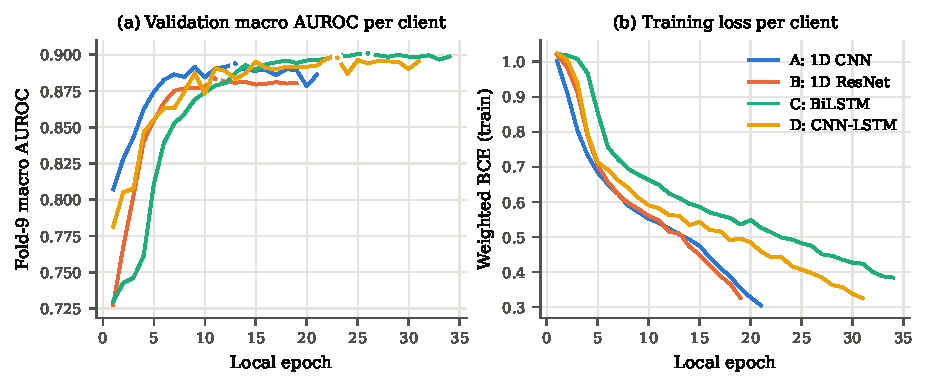
\includegraphics[width=0.9\textwidth]{client_curves}
\caption{Local training of the four clients (seed 42): (a) fold-9 macro AUROC per epoch, with the
selected epoch marked by a dot; (b) class-weighted training BCE per epoch. Each curve ends when early
stopping (patience 8) was triggered.}
\label{fig:clientcurves}
\end{figure*}

\begin{table*}[!t]
\centering
\caption{Client-wise training summary (mean over 3 seeds; loss and AUROC mean $\pm$ SD at the selected epoch)}
\label{tab:clienttrain}
\footnotesize
\begin{tabular}{@{}lcccccc@{}}
\toprule
Model & $n_{\text{train}}$ & Epochs run & Best epoch & Train loss & Fold-9 AUROC & $T_i$ \\
\midrule
Client A & 4{,}277 & 20.7 & 12.7 & 0.510 $\pm$ 0.036 & 0.893 $\pm$ 0.001 & 1.74 $\pm$ 0.22 \\
Client B & 4{,}280 & 21.7 & 13.7 & 0.479 $\pm$ 0.079 & 0.886 $\pm$ 0.002 & 1.52 $\pm$ 0.15 \\
Client C & 4{,}264 & 35.0 & 27.0 & 0.466 $\pm$ 0.017 & 0.900 $\pm$ 0.001 & 1.25 $\pm$ 0.09 \\
Client D & 4{,}263 & 30.7 & 22.7 & 0.450 $\pm$ 0.024 & 0.898 $\pm$ 0.001 & 1.35 $\pm$ 0.06 \\
Pooled (folds 1--8) & 17{,}084 & 31.0 & 23.0 & 0.452 $\pm$ 0.037 & 0.914 $\pm$ 0.002 & 1.31 $\pm$ 0.08 \\
\bottomrule
\end{tabular}

\end{table*}

The convolutional clients converge fastest: Client A reaches its best validation AUROC after 12.7
epochs and Client B after 13.7 epochs on average, after which the validation AUROC stagnates or
decreases while the training loss keeps falling, the typical sign of over-fitting on a small local
dataset. The recurrent clients learn more slowly at the start (Client C stays below 0.80 for the
first four epochs in Fig.~\ref{fig:clientcurves}a) but keep improving for longer, with best epochs
of 27.0 (C) and 22.7 (D), and they end with the highest validation AUROCs (0.900 and 0.898). The
fitted temperatures are all larger than one (1.25--1.74 on average), i.e.\ every client is
over-confident after training with the class-weighted loss, and calibration is therefore needed before
probabilities from different clients can be averaged meaningfully.

\subsubsection{Global Model (Server) Test Accuracy and Loss}
The server performs no iterative training, so there are no communication rounds over which a server
accuracy or loss could converge. The closest analogue is the behaviour of the global model as client
contributions are added. Fig.~\ref{fig:server} plots the macro AUROC of the equal-weight global model
against the number of aggregated clients, both on fold 9 and on the test fold. Both curves rise
monotonically and flatten after three clients: the mean over all subsets increases from 0.890 with
one client to 0.900 with two, 0.903 with three and 0.905 with four on the test fold. The gap between
the fold-9 and the test curves remains small (0.004 for the full federation), which shows that the
validation-based selection did not over-fit the gate. In terms of loss, the selected gate has a
cross-validated binary cross-entropy of 0.372 on fold 9 and a test binary cross-entropy of 0.376
$\pm$ 0.008; the learned static (0.349 $\pm$ 0.004) and dynamic (0.343 $\pm$ 0.005) gates have lower
test losses, mirroring their better calibration on fold 9 (Table~\ref{tab:fusion}), but a lower AUROC.

\begin{figure}[!t]
\centering
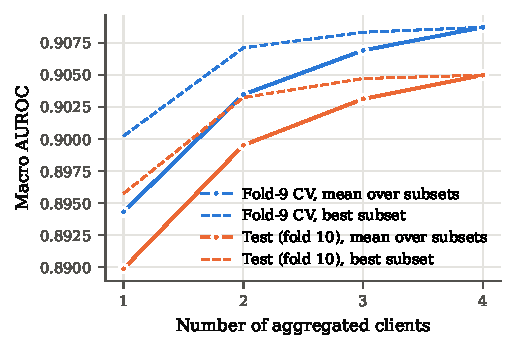
\includegraphics[width=\columnwidth]{server_convergence}
\caption{Macro AUROC of the global (server) model as a function of the number of aggregated clients,
averaged over all subsets of that size (solid) and for the best subset (dashed).}
\label{fig:server}
\end{figure}

\subsubsection{Comparison with Other Federated Learning Frameworks}
Parameter-averaging frameworks cannot combine the heterogeneous clients of CardioSentinel, so they were
evaluated with one shared architecture, the CNN-LSTM of Client~D, on exactly the same four client
partitions. FedAvg \cite{mcmahan2017fedavg}, FedProx \cite{li2020fedprox} ($\mu=0.01$), SCAFFOLD
\cite{karimireddy2020scaffold} (control variates, option II) and FedNova \cite{wang2020fednova}
(updates normalised by the number of local steps) were run for 20 communication rounds of one local
epoch each, with the client recipe of Section~\ref{sec:setup} (AdamW, learning rate $10^{-3}$, batch
128, class-weighted loss, augmentation, gradient clipping) and aggregation weights $n_k/n$. The round
with the best fold-9 macro AUROC was kept, calibrated and thresholded on fold 9, and evaluated once on
the test fold. Because of the computational cost these runs use seed 42 only, so
Table~\ref{tab:fedcomp} reports seed-42 values for every row, and Fig.~\ref{fig:flconv} shows the
convergence.

\begin{table}[!t]
\centering
\caption{Comparison with federated-learning frameworks on the same four client partitions (seed 42;
test fold unless stated). $^{a}$Patient-grouped CV on fold 9.}
\label{tab:fedcomp}
\footnotesize
\setlength{\tabcolsep}{3pt}
\resizebox{\columnwidth}{!}{\begin{tabular}{@{}lcccccc@{}}
\toprule
Method & Rounds & Same arch. & Fold-9 AUROC & Test AUROC & F1 (\%) & Acc. (\%) \\
\midrule
Local only (best client, D) & 0 & -- & 0.898 & 0.895 & 68.9 & 85.0 \\
FedAvg \cite{mcmahan2017fedavg} & 20/20 & yes & 0.911 & 0.907 & 71.8 & 87.2 \\
FedProx ($\mu=0.01$) \cite{li2020fedprox} & 20/20 & yes & 0.910 & 0.906 & 71.4 & 86.9 \\
SCAFFOLD \cite{karimireddy2020scaffold} & 1/20 & yes & 0.850 & 0.842 & 62.4 & 80.6 \\
FedNova \cite{wang2020fednova} & 20/20 & yes & 0.911 & 0.907 & 71.5 & 86.8 \\
\textbf{Proposed (one-shot gate)} & 1 & no & 0.908\textsuperscript{a} & 0.905 & 70.9 & 86.8 \\
\midrule
Centralised (pooled data) & -- & -- & 0.916 & 0.909 & 69.6 & 85.5 \\
\bottomrule
\end{tabular}
}
\end{table}

\begin{figure*}[!t]
\centering
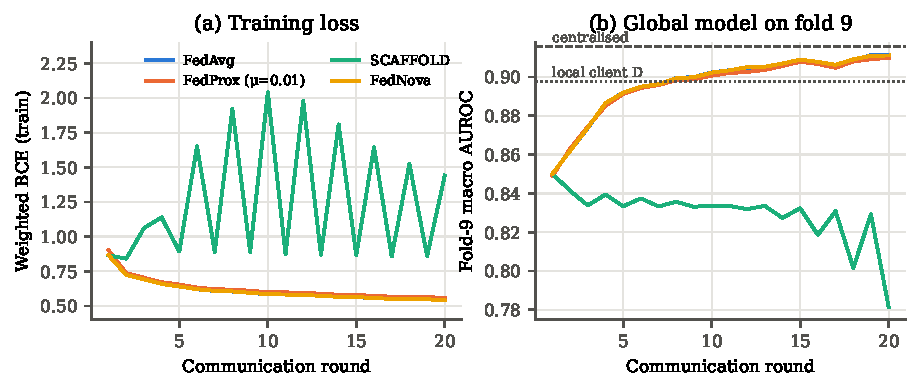
\includegraphics[width=0.9\textwidth]{fl_convergence}
\caption{Convergence of the parameter-averaging frameworks (shared CNN-LSTM, seed 42): (a) training
loss averaged over clients; (b) fold-9 macro AUROC of the global model, with the local-only Client D
and the centrally trained CNN-LSTM as references.}
\label{fig:flconv}
\end{figure*}

\textit{Accuracy.} FedAvg and FedNova reach a test macro AUROC of 0.907 and FedProx 0.906, slightly
above the proposed one-shot gate (0.905) and close to centralised training (0.909). They also achieve a
higher macro F1 (71.4\%--71.8\% versus 70.9\%). With identical clients and many communication rounds,
parameter averaging thus remains marginally more accurate than prediction-level aggregation; the
difference to the proposed model (0.002 AUROC) is, however, smaller than the gain of either approach
over local training (0.895 for Client~D in this seed). SCAFFOLD failed in this configuration: its best
global model was the one after the first round (test AUROC 0.842), and its training loss oscillated
between about 0.8 and 2.0 in subsequent rounds. The control-variate correction assumes plain SGD
local steps of size $\eta$, and combined with the adaptive AdamW updates used here it over-corrects
the client drift; with SGD local training it may behave differently.

\textit{Stability and convergence speed.} FedAvg, FedProx and FedNova converge smoothly and almost
identically (Fig.~\ref{fig:flconv}): they pass the local-only reference of 0.898 on fold 9 at round 8, exceed 0.90 at round 10 and are still improving slightly at round 20, so more rounds could add
a little more. FedNova coincides with FedAvg because all four clients perform the same number of local
steps (33 per epoch), in which case its normalisation has no effect; the proximal term of FedProx is
unnecessary when the label distributions of the clients are as similar as here. The cost of this
accuracy is communication and coordination: 20 synchronised rounds, each exchanging the full set of
0.47M parameters with every client, and the requirement that all institutions train the same network.
The proposed model needs a single round, exchanges only five probabilities per client and query, and
lets every institution keep its own architecture, at a cost of about 0.002 AUROC in this setting.

% ---------------------------------------------------------------------------------- F
\subsection{Class-wise Analysis}
\label{sec:classwise}

\subsubsection{Confusion Matrix}
Fig.~\ref{fig:confusion} shows the per-class confusion matrices of the proposed model on the 2,158
test records for seed 42, at the thresholds chosen on fold 9 (0.42 for NORM, 0.62 for MI and STTC
and 0.64 for CD and HYP), and Fig.~\ref{fig:roc} the corresponding ROC curves. Because the task is
multi-label, each superclass has its own $2\times2$ matrix.

\begin{figure*}[!t]
\centering
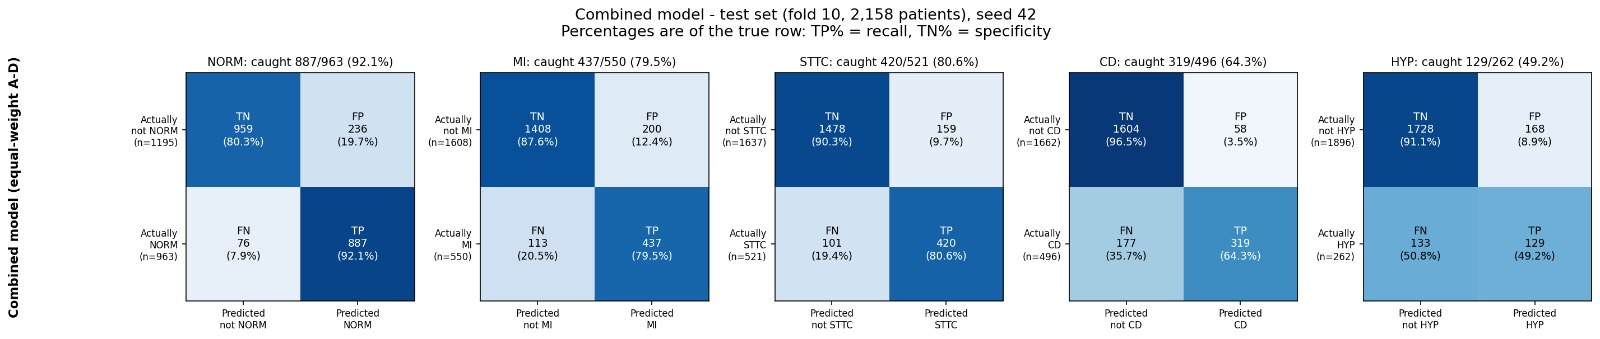
\includegraphics[width=\textwidth]{confusion_combined.jpg}
\caption{Per-class confusion matrices of the proposed model on the test fold (seed 42); counts and
row-normalised rates (TP\% = recall, TN\% = specificity).}
\label{fig:confusion}
\end{figure*}

\begin{figure}[!t]
\centering
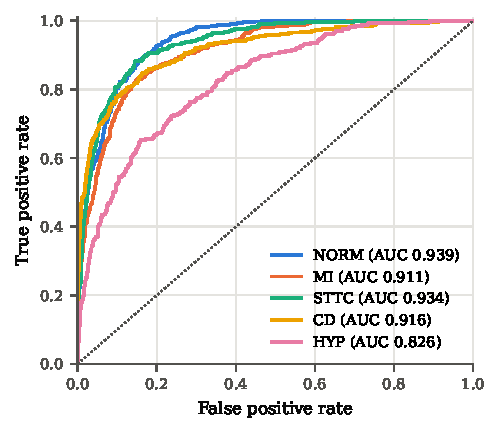
\includegraphics[width=0.9\columnwidth]{roc}
\caption{ROC curves of the proposed model on the test fold for the five superclasses (seed 42).}
\label{fig:roc}
\end{figure}

NORM is detected most reliably: 887 of its 963 positives are found (recall 0.92), at the cost of 236
false positives, which reflects the low NORM threshold that favours sensitivity. For STTC and MI the
model identifies 420 of 521 and 437 of 550 positives, with 159 and 200 false positives respectively.
CD is predicted conservatively: only 58 false positives occur, but 177 of the 496 positives are
missed. HYP is the most difficult class, with 129 true positives, 133 false negatives and 168 false
positives; hypertrophy criteria rely on voltage amplitudes, which the per-recording z-scoring
partly removes, and HYP frequently co-occurs with STTC and CD, so its ECG changes overlap with those
of other classes. The ROC curves confirm this ranking, with the HYP curve clearly below the others.

Compared with the four clients, each at its own fold-9 thresholds (seed 42), for MI the
gate both finds the most positives (437 against 408--431) and raises the fewest false alarms (200
against 226--258). For CD it trades recall for precision: the clients find 314--355 positives with
110--163 false positives, the gate 319 with only 58. The gain of the combination is therefore mainly
in precision, in line with Table~\ref{tab:main}, where the macro precision rises from at most 67.0\%
to 69.8\% while the recall stays at the level of the clients.

\subsubsection{Class-wise Performance Table}
Table~\ref{tab:classwise} reports precision, recall, F1-score and AUROC per superclass, averaged over
the three seeds, together with the macro and support-weighted averages.

\begin{table}[!t]
\centering
\caption{Class-wise performance of the proposed model on the test fold (mean of 3 seeds)}
\label{tab:classwise}
\footnotesize
\setlength{\tabcolsep}{4pt}
\begin{tabular}{@{}lccccc@{}}
\toprule
Class & Precision & Recall & F1-score & AUROC & Support \\
\midrule
NORM & 0.782 & 0.930 & 0.850 & 0.938 & 963 \\
MI & 0.724 & 0.730 & 0.725 & 0.912 & 550 \\
STTC & 0.745 & 0.792 & 0.768 & 0.933 & 521 \\
CD & 0.800 & 0.682 & 0.735 & 0.914 & 496 \\
HYP & 0.439 & 0.490 & 0.461 & 0.828 & 262 \\
\midrule
Macro avg. & 0.698 & 0.725 & 0.707 & 0.905 & 2792 \\
Weighted avg. & 0.735 & 0.780 & 0.753 & 0.917 & 2792 \\
\bottomrule
\end{tabular}

\end{table}

NORM (F1 0.850) and STTC (0.768) are the best-recognised superclasses, followed by CD (0.735) and MI
(0.725). HYP remains clearly weaker (F1 0.461, AUROC 0.828), and because it is also the rarest class
it pulls the macro F1 (0.707) below the support-weighted F1 (0.753). The AUROC of every class except
HYP exceeds 0.91, so the ranking quality is high and the lower F1 values of MI and CD are largely a
matter of operating point.

Fig.~\ref{fig:confusion-mean} gives the confusion matrices averaged over the three seeds. Summed over
the five classes, the model makes 2,177 true-positive and 7,198 true-negative decisions out of 10,790
(2,158 ECGs $\times$ 5 classes), a label-wise accuracy of 0.869 with a micro-averaged precision of
0.731 and recall of 0.780; the 615 false negatives are dominated by HYP (134), CD (158) and MI (148).

\begin{figure*}[!t]
\centering
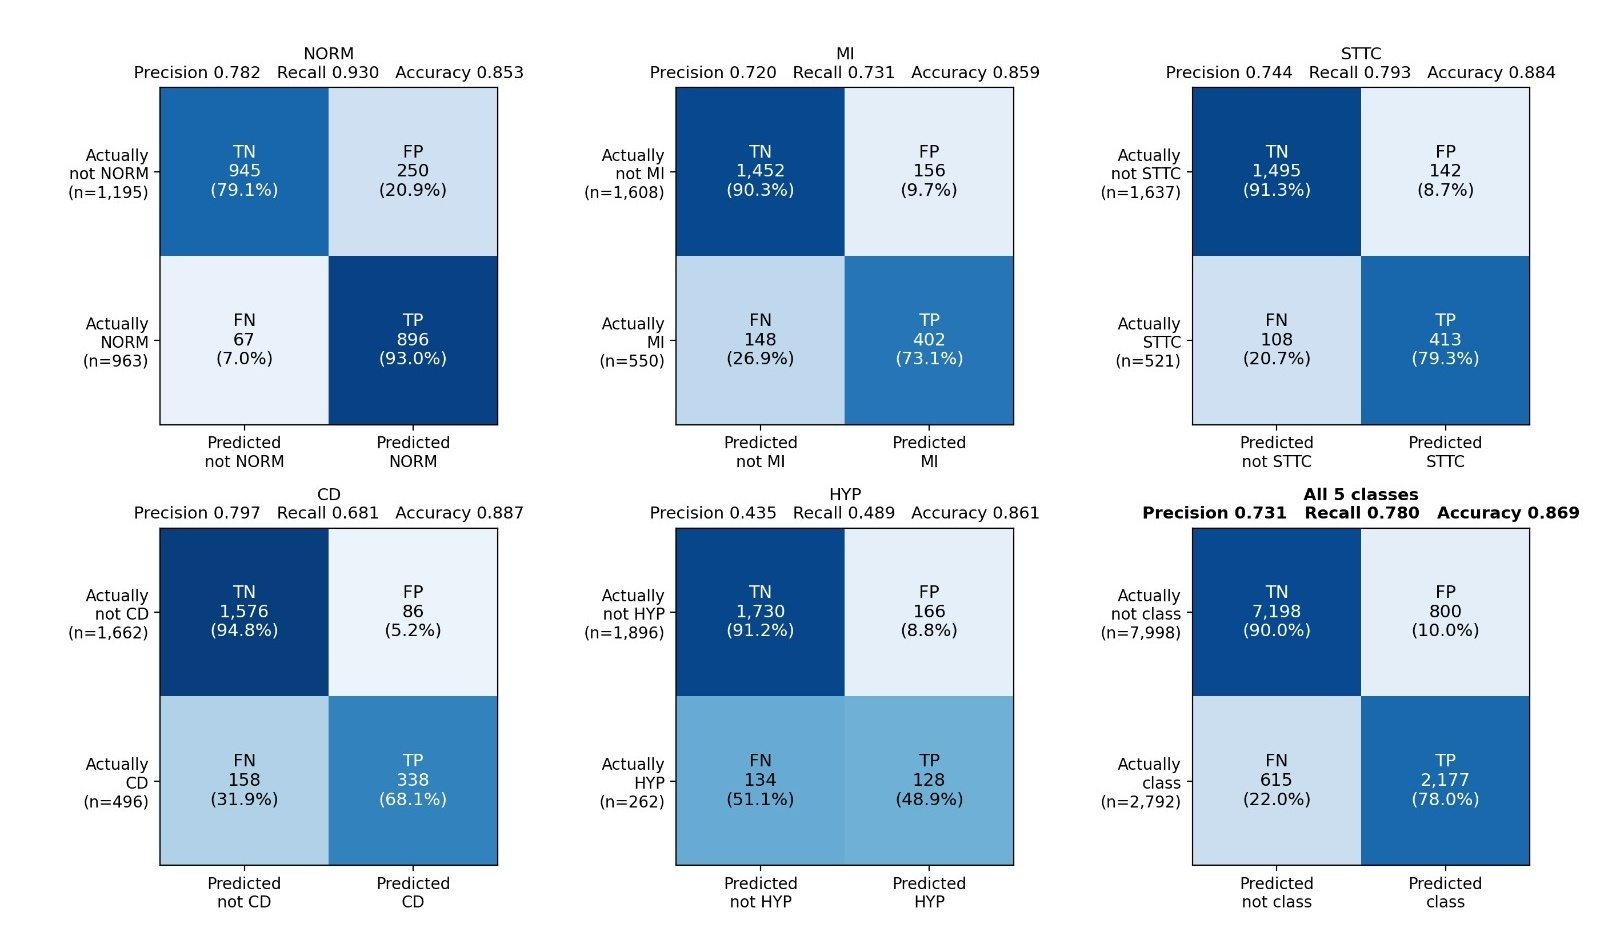
\includegraphics[width=0.85\textwidth]{confusion_mean.jpg}
\caption{Per-class confusion matrices of the proposed model on the test fold (fold 10, 2,158 ECGs), mean
counts over seeds 42, 43 and 44; percentages are of the true row. The last panel sums the five classes
(2,158 ECGs $\times$ 5 decisions = 10,790).}
\label{fig:confusion-mean}
\end{figure*}

\textit{Per-finding triage.} When the clinical requirement is a precision and recall of at least 0.90,
no global threshold can satisfy it for all classes. Applying the rule-in/rule-out bands fitted on
fold 9 (Section~\ref{sec:clf}) to the test fold, 53.7\% of all findings are decided automatically,
with a macro precision of 0.937, a macro recall of 0.908 over the automated classes and an accuracy of
0.967; 17.8\% of the ECGs are decided completely without referral. NORM, MI and CD were automated in
all seeds, STTC in one of three seeds, and HYP only in rule-out mode, so every possible HYP finding is
referred. Not every target was met: the test recall of CD was 0.880.

% ---------------------------------------------------------------------------------- G
\subsection{Explainable Results}
\label{sec:xai-results}

The explanations were computed for the selected equal-weight gate of seed 42 on 300 randomly drawn
validation (fold-9) records, which contain 131 NORM, 81 MI, 65 STTC, 80 CD and 31 HYP positives;
the test fold was not used. Fig.~\ref{fig:xaileads} shows the global lead importance, i.e.\ the share
of the absolute Integrated-Gradients attribution falling on each lead, averaged over the positive
records of each class. Under a uniform distribution every lead would receive 8.3\%.

\begin{figure}[!t]
\centering
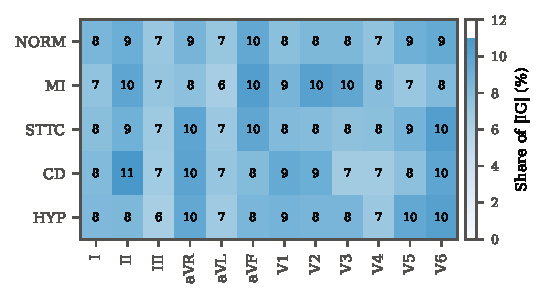
\includegraphics[width=\columnwidth]{xai_leads}
\caption{Global explanation: share of the absolute Integrated-Gradients attribution per lead (\%)
for the positive validation records of each superclass (seed 42, equal-weight gate).}
\label{fig:xaileads}
\end{figure}

The attributions are spread over all twelve leads (no lead receives more than 11.0\%), which is
consistent with the redundancy of the leads shown in Fig.~\ref{fig:leadcorr} and with training under
lead dropout. Within this spread the emphasis follows the expected anatomy. For MI the largest shares
fall on aVF (10.3\%), V2 (10.1\%), II (9.8\%) and V3 (9.7\%), i.e.\ on the inferior and anteroseptal
leads that record the most frequent infarct locations. For HYP the largest shares fall on V6
(10.3\%), V5 and aVR (9.6\% each) and V1 (8.6\%), the leads used by the classical voltage criteria
for left ventricular hypertrophy, which combine the S wave in V1 with the R wave in V5 or V6. For CD
the model relies most on II (11.0\%), aVR (9.9\%), V6 (9.8\%) and V1 (9.4\%); V1 and V6 are the leads
in which right and left bundle branch blocks are recognised. STTC is attributed mainly to the
lateral and inferior leads V6 (10.3\%), aVR (9.8\%) and aVF (9.7\%). In every class, leads III and aVL
are among the four least-attributed leads (6.2\%--7.2\%); both are linear combinations of I and II,
so they add little independent information.

\textit{Local explanations.} Fig.~\ref{fig:xailocal} shows the two validation records predicted with
the highest confidence for MI and for STTC, with the three leads that carry the largest attribution
and the attribution magnitude along time. Record 5927 (label MI) is classified as MI with probability
0.99, and its attribution concentrates on V2, V3 and V4. These leads show deep, predominantly negative
QRS complexes, the pattern of an anterior infarction, and the attribution peaks at each QRS complex
rather than in the baseline between beats. Record 14758 (labels STTC and HYP) receives P(STTC) = 0.98
and P(HYP) = 0.85, so both of its labels are recovered; for STTC the attribution falls on V2, V1 and
aVF and again peaks at the QRS complexes and the adjoining ST segments of the beats. In both cases the
attribution is locked to the beats and falls on the waveform segments a cardiologist would inspect,
not on the baseline between beats; two examples cannot, however, establish this for all records.

\begin{figure*}[!t]
\centering
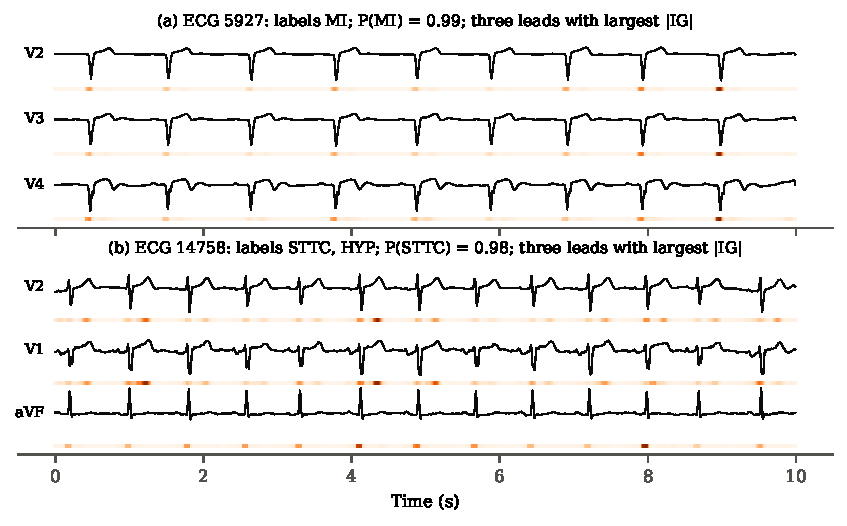
\includegraphics[width=0.95\textwidth]{xai_local}
\caption{Local explanations for the most confident true-positive (a) MI and (b) STTC validation
records. For each record the three leads with the largest total attribution are shown; the colour
strip below each trace encodes $|\mathrm{IG}|$ over time (darker = larger), smoothed over 90~ms.}
\label{fig:xailocal}
\end{figure*}

\textit{Faithfulness.} Table~\ref{tab:deletion} reports the deletion test. For NORM, MI and CD,
removing the lead with the largest attribution lowers the mean predicted probability more than
removing a random lead (NORM: $-$0.028 versus $-$0.019; MI: $-$0.030 versus $-$0.006; CD: $-$0.043
versus $-$0.012), and removing the three most important leads lowers it substantially more than
removing three random leads (NORM: $-$0.135 versus $-$0.074; MI: $-$0.057 versus $-$0.006; CD:
$-$0.070 versus $-$0.009). For these classes the attributions therefore identify leads on which the
prediction actually depends. For STTC and HYP, in contrast, neither targeted nor random deletion
changes the probability appreciably (STTC: 0.764 intact, 0.765--0.772 after deletion; HYP: 0.620
intact, 0.613--0.627 after deletion). The evidence for these two classes is distributed redundantly
over many leads, so lead-level attributions should not be read as identifying a single decisive lead.

\begin{table}[!t]
\centering
\caption{Deletion test: mean gate probability of the true class after zeroing the $k$ leads with the
largest IG attribution or $k$ random leads (fold-9 positives, seed 42)}
\label{tab:deletion}
\footnotesize
\setlength{\tabcolsep}{4pt}
\resizebox{\columnwidth}{!}{\begin{tabular}{@{}lcccccc@{}}
\toprule
 & & & \multicolumn{2}{c}{Top-$k$ IG leads removed} & \multicolumn{2}{c}{Random $k$ leads removed} \\
\cmidrule(lr){4-5}\cmidrule(l){6-7}
Class & $n$ & Mean $p$ (intact) & $k=1$ & $k=3$ & $k=1$ & $k=3$ \\
\midrule
NORM & 131 & 0.741 & 0.713 & 0.606 & 0.722 & 0.667 \\
MI & 81 & 0.750 & 0.720 & 0.693 & 0.744 & 0.744 \\
STTC & 65 & 0.764 & 0.765 & 0.772 & 0.764 & 0.771 \\
CD & 80 & 0.758 & 0.715 & 0.688 & 0.746 & 0.749 \\
HYP & 31 & 0.620 & 0.626 & 0.621 & 0.627 & 0.613 \\
\bottomrule
\end{tabular}
}
\end{table}

\textit{Federation-level explanation.} At the level of the institutions, the Shapley values in
Table~\ref{tab:shapley} show that the four clients contribute comparably to the AUROC of the
federation (0.097--0.105 on the test fold), with the recurrent clients C and D contributing most.
Together with the signal-level attributions, this gives a clinician two complementary views: which
leads and waveform segments drove a finding, and which participating sites the global model relied on.
These explanations are post hoc and were not yet reviewed by cardiologists, and IG with a zero
baseline, like every attribution method, depends on the choice of baseline.


% ---------------------------------------------------------------------------------- H
\subsection{Comparison with State-of-the-Art and Discussion}
\label{sec:discussion}

Table~\ref{tab:sota} compares the proposed model with published results on the PTB-XL superclass
task. The models of \cite{strodthoff2021} were trained centrally on the same folds 1--8 and tested on
the same fold 10, and they are therefore the most directly comparable; the other entries use the
same superclass labels but different training protocols.

\begin{table}[!t]
\centering
\caption{Comparison with state-of-the-art results on the PTB-XL five-superclass task}
\label{tab:sota}
\footnotesize
\setlength{\tabcolsep}{3pt}
\begin{tabular}{@{}p{3.2cm}p{1.6cm}cc@{}}
\toprule
Method & Training data & Macro AUROC & Acc.\ (\%) \\
\midrule
Wavelet + NN \cite{strodthoff2021} & pooled & 0.874 & -- \\
inception1d \cite{strodthoff2021} & pooled & 0.921 & -- \\
LSTM (bidir.) \cite{strodthoff2021} & pooled & 0.921 & -- \\
xresnet1d101 \cite{strodthoff2021} & pooled & 0.928 & -- \\
resnet1d\_wang \cite{strodthoff2021} & pooled & 0.930 & -- \\
Ensemble \cite{strodthoff2021} & pooled & 0.934 & -- \\
ST-MEM \cite{na2024stmem} & pooled + pretrain & 0.933 & 82.5 \\
METS, zero-shot \cite{li2023mets} & pooled + text & -- & 84.2 \\
\midrule
Pooled CNN-LSTM (ours) & pooled & 0.909 & 86.4 (label) \\
XGBoost, 172 features (ours) & pooled & 0.909 & 86.8 (label) \\
FedAvg, CNN-LSTM (ours, seed 42) & 4 sites, 20 rounds & 0.907 & 87.2 (label) \\
\textbf{Proposed (federated)} & 4 sites, 1 round & \textbf{0.905} & \textbf{86.9 (label)} \\
\bottomrule
\end{tabular}
\end{table}

The proposed model does not exceed the best centrally trained models: its macro AUROC of 0.905 is
0.016--0.029 below the centrally trained deep networks and the ensemble of
\cite{strodthoff2021}. Part of
this gap is attributable to the data restriction, since each client sees only 25\% of the training
records, and part to the training recipe, since our own pooled CNN-LSTM reaches 0.909 rather than
0.92--0.93; the recipe (100~Hz input, no test-time augmentation, no external pretraining) was kept
fixed for all models to isolate the effect of federation. The accuracies in Table~\ref{tab:sota} are
not directly comparable either, because ST-MEM and METS report accuracy under their own definitions, whereas the
label-wise accuracy of this work averages the five binary decisions.

\textit{Strengths.} The main strength of the approach is that it delivers most of the benefit of
pooling the data without moving any record or parameter: the federated gate recovers about 70\% of the
AUROC lost by splitting the data and ties the pooled CNN-LSTM in macro F1, with one communication step
and freely chosen architectures. It outperforms every model that can be trained at a single site,
including XGBoost on hand-crafted features (0.898 on average), and comes within 0.002 AUROC of FedAvg,
which needs twenty synchronised rounds and a common architecture. The improvement over the best institution is statistically
significant in every seed, the results are highly reproducible (the SD of the gate's macro AUROC over
seeds is below 0.001), and all modelling choices, including the aggregation rule, were made on
validation data before a single evaluation on the test fold. The triage rule converts the model into a
tool that decides about half of all findings automatically at a precision above 0.93, while stating
explicitly which findings require a cardiologist.

\textit{Limitations.} First, the four clients are simulated partitions of one dataset from one
hospital system with near-identical label distributions, so the benefits of the method under real
inter-site shifts (different devices, populations and label practices) remain to be shown. Second,
fold 9 is used for early stopping, calibration, thresholds and the gate, so validation figures are
optimistic; only the test-fold figures are unbiased. Third, the learned gates did not improve on
equal weighting, which suggests that the per-patient gate lacks informative inputs when all clients
see the same signal. Fourth, HYP remains poorly recognised, and the bootstrap confidence intervals
resample records rather than patients (the test fold contains 2,158 records from 1,877 patients).
Fifth, two baselines are stronger than the proposed model: parameter averaging with a shared
CNN-LSTM (FedAvg and FedNova, 0.907) and, without any federation, XGBoost on hand-crafted features
trained on the pooled data (0.909, macro F1 72.6\%). The latter shows that absolute amplitude features,
which the deep clients do not see, carry information that the current gate cannot exploit; adding a
feature-based client to the federation is an obvious extension. Finally, the federated baselines and the
activation and optimizer ablations were run with a single seed, and the triage and explanation analyses
use seed 42.

\textit{Why federation helps.} The federation helps for two reasons. It enlarges the effective
training set without data sharing: no single client can learn from more than a quarter of the
records, but the gate combines models that together have seen all of them. And because the clients
use different architectures, their errors are only partly correlated, so averaging their calibrated
probabilities reduces variance in the same way as a deep ensemble \cite{lakshminarayanan2017,dietterich2000ensemble}:
every pair of clients already outperforms every single client, even though no client was trained to
complement the others.
